% Generated by analyze_t8.js - paragraph and figure for Section 5
\subsection{Effect of Supply-Chain Complexity}
\label{sec:eval-complexity}

To assess how the mechanisms scale with the structure of the supply chain, we measured, under sequential submission,
(a)~a transformation merging $n \in \{1, 5, 10, 25, 50, 100\}$ input lots, followed by packaging, binding, verification and
consumption of the resulting certificate, and (b)~chains of $d \in \{1, 5, 10, 20\}$ successive transformations
before packaging (Figure~\ref{fig:eval-complexity}). The cost of a transformation grows linearly with its number of inputs, by 2.29\,ms of chaincode execution
per input lot ($R^2 = 1.00$), from 29.0\,ms for one lot to 257.0\,ms for 100, since mass
balance and input consumption read and update every input. The binding of the resulting certificate, which embeds the list of inputs,
took 29.7\,ms for one input and 27.2\,ms for 100, and UID verification 11.5 and
8.5\,ms respectively.  With 20 upstream transformations, binding took 23.5\,ms and verification 9.5\,ms, against
27.9 and 8.0\,ms with a single one. In all cases the end-to-end latency
remained dominated by block cutting.

\begin{figure}[t]
\centering
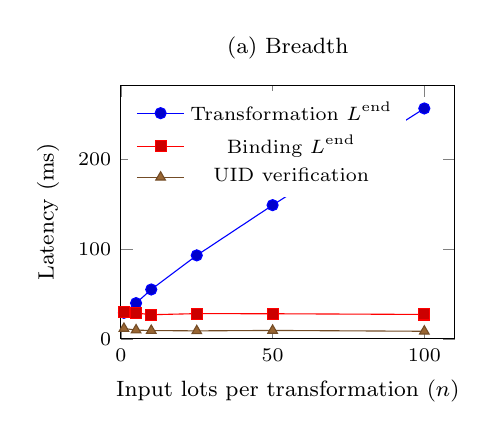
\begin{tikzpicture}
\begin{axis}[width=0.48\linewidth, height=4.8cm, xlabel={Input lots per transformation ($n$)}, ylabel={Latency (ms)},
  xmin=0, ymin=0, tick label style={font=\scriptsize}, label style={font=\footnotesize},
  legend style={font=\scriptsize, at={(0.02,0.98)}, anchor=north west, draw=none}, title={(a) Breadth}, title style={font=\footnotesize}]
\addplot+[mark=*] coordinates {(1,29.00) (5,39.85) (10,55.07) (25,93.12) (50,149.15) (100,257.02)};
\addlegendentry{Transformation $L^{\mathrm{end}}$}
\addplot+[mark=square*] coordinates {(1,29.66) (5,28.82) (10,26.91) (25,28.13) (50,27.99) (100,27.22)};
\addlegendentry{Binding $L^{\mathrm{end}}$}
\addplot+[mark=triangle*] coordinates {(1,11.52) (5,9.80) (10,9.26) (25,8.89) (50,9.37) (100,8.45)};
\addlegendentry{UID verification}
\end{axis}
\end{tikzpicture}\hfill
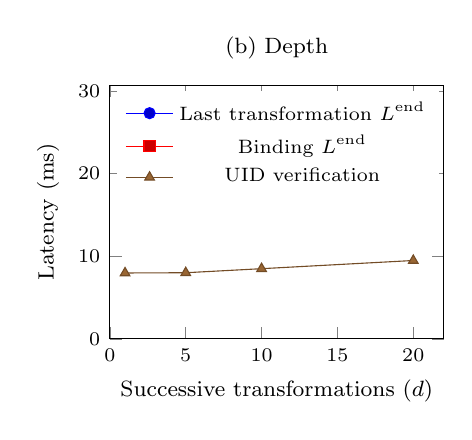
\begin{tikzpicture}
\begin{axis}[width=0.48\linewidth, height=4.8cm, xlabel={Successive transformations ($d$)}, ylabel={Latency (ms)},
  xmin=0, ymin=0, tick label style={font=\scriptsize}, label style={font=\footnotesize},
  legend style={font=\scriptsize, at={(0.02,0.98)}, anchor=north west, draw=none}, title={(b) Depth}, title style={font=\footnotesize}]
\addplot+[mark=*] coordinates {(1,24.08) (5,18.50) (10,18.56) (20,19.31)};
\addlegendentry{Last transformation $L^{\mathrm{end}}$}
\addplot+[mark=square*] coordinates {(1,27.88) (5,23.41) (10,26.34) (20,23.51)};
\addlegendentry{Binding $L^{\mathrm{end}}$}
\addplot+[mark=triangle*] coordinates {(1,7.97) (5,8.00) (10,8.49) (20,9.48)};
\addlegendentry{UID verification}
\end{axis}
\end{tikzpicture}
\caption{Cost as a function of supply-chain complexity (sequential submission, mean values): (a) one transformation with
$n$ input lots; (b) a chain of $d$ successive transformations before packaging and binding.}
\label{fig:eval-complexity}
\end{figure}
